\chapter{Related approaches for real-valued problem optimization}
\label{ch:Approaches-for-real-valued-problem}

This chapter introduces two techniques for real-valued function optimization
based on evolution computation in Section~\ref{sec:rECGA} and Section~\ref{sec:CMA-ES}.
In Section~\ref{sec:motivation}, the difficulty of CMA-ES is introduced and the
hypothesis of this thesis to conquer the hazard is then proposed.

Due to the difficulties introduced in the previous chapter, it is considered
appropriate to apply stochastic algorithms to avoid some of the described
hazards.  Many approaches has been proposed for real-valued problem
optimization.  For example, Ant colony optimization (ACO), Bat algorithm (BA),
Differential evolution (DE).  Among the famous optimization methods, estimation
of distribution algorithms (EDAs)~\cite{Pelikan:2012:EDA} and evolution strategies (ESs) are two major
branches of evolution computation and both have performed well on optimization
problems.  They will be introduced respectively in this chapter along with
useful solution to real-valued function optimization. 


\section{Real-coded extended compact genetic algorithm}
\label{sec:rECGA}

Real-coded extended compact genetic algorithm (rECGA) is a modification
of extended compact genetic algorithm (ECGA)~\cite{Harik:1999:ecga}, which belongs to the
family of EDAs.  ECGA being a well-known EDA can only solve problems in
discrete domain due to the assumption of the problem encoding.  As a
result, rECGA is interested in the ability of model building in ECGA and
wants to do some modification to make ECGA compatible with real-valued
problems.  The main framework of rECGA is to integrate discretization
techniques into ECGA so that ECGA can cope with problems in continuous
domain.  \subsection{EDAs}

The term \emph{linkage} in the genetic algorithm
(GA)~\cite{Holland:1975}~\cite{Goldberg:1989:ga-book} field illustrates
the dependency among variables, while \emph{building blocks} (BBs)
refers to groups of related groups.  Many techniques have been developed
to cope with the linkage problems since Holland lays emphasis on the
importance of BBs.  Studies have shown that the scalable performance of
GA can only be obtained when building block information is already in
the problem coding or given before or the
search~\cite{thierens1999scalability}.  Therefore, linkage
learning is the key to make an optimization procedure competent.

EDAs, sometimes also called probabilistic model-building genetic algorithms
(PMBGAs), are stochastic optimization methods that build models
explicitly on selected candidate solutions iteratively.
We perform a selection on population and extract the information of
selected individuals by building model.
At the end of each iteration, a new population is generated accordingly.
The main difference between EDAs and conventional evolution algorithms
is that other evolution algorithms use implicit models to generate
solutions, while EDAs construct an explicit model to represent the
promising population obtained so far and sample new solutions
accordingly.
EDAs play an important role in optimization problems because the
probabilistic model is able to extract previously unknown problem
information.  Moreover, some advanced EDAs like ECGA, are able to
further illustrate the linkage information among the decision variables.

EDAs can be algorithmically outlined as Algorithm~\ref{algo:EDA}.


\begin{algorithm}

  \While{termination criteria is not met}{
  Initialize population randomly\;
  select promising individuals from current population\; 
    build probabilistic model using selected individuals\;
    \If{model converges} { break\; }
    sample from the model to generate new individuals\;
    replace the
    previous population by the sampled	individuals\;
  } \caption {EDAs()}
  \label{algo:EDA} 
 \end{algorithm}

There are many different EDAs using different methods to build
probabilistic models.  Better-known EDAs are univariate marginal
distribution algorithm (UMDA), extended compact genetic algorithm
(ECGA), bayesian optimization algorithm (BOA), etc.

ECGA is proposed by Harik in 1999.
The main concept of ECGA comes from that a good probabilistic model
inspires good linkage learning.
Based on the idea, what should be figured out next is the definition of
a good probabilistic model.
The procedure for model building in ECGA is describes as
Algorithm~\ref{algo:ecga}, and we can further describe the concept in
Figure~\ref{fig:model building}.
When building model, we first regard each decision variable as a group.
By greedily testing if we can better describe the model by merging two
groups, ECGA keeps finding if there is a better merging.
In the example, we believe that the joint probability is with the
following form:
\[Pr(x_1,x_2,x_3,x_4) = Pr(x_1)Pr(x_2,x_4)Pr(x_3).\]
In other words, we believe that merging $x_2$ and $x_4$ better describes
this model.

The overall procedure of ECGA can be illustrated as Figure~\ref{fig:ecgaflow}.
Starting from initialization, selection is performed followed by model
building.
The offspring are generated according to the model and measurement for
convergence of offspring takes place.
If the termination criteria is met, the procedure terminates; otherwise,
the offspring are used for selection for the beginning of next
iteration.

\begin{figure}[htpb]
  \centering
  \includegraphics[bb=50 73 777 554, clip, width=.9\textwidth]{ECGA.eps}
  \caption{Flow of ECGA}
  \label{fig:ecgaflow}
\end{figure}

\begin{figure}[htpb]
  \centering
  \includegraphics[bb= 32 150 552 450, clip, width =0.4\textwidth]{modelbuilding.eps}
  \caption{Model Building in ECGA}
  \label{fig:model building}
\end{figure}
\begin{algorithm}  \KwData{MPM with $\ell$ groups, each contains one
  variable, where $\ell$ is the problem size } \While{there is a pair
  which can reduce CCC} { Finding one pair greedily which reduces CCC
    the most \; merge the pair\; } \caption{model building in ECGA}
    \label{algo:ecga}
  \end{algorithm}

However, ECGA proposed by Harik focuses on bitstring problems while
continuous problems are not solved yet.  To optimize a real-valued
function, ECGA have to overcome the problem of compatibility.
Therefore, the concept of discretization is introduced to make
real-valued optimization problems fit the encoding of ECGA.  After
transforming the problem from continuous domain to discrete domain, the
target of the problem is meanwhile changed from optimizing the quality
of solutions to finding a more feasible solution which optima may
locate.  The template of integrating the discretization method into ECGA
is the so-called real-coded extended compact genetic algorithm (rECGA).
Two traditional discretization methods are introduced in the following
section, and a modified one along with the integration into ECGA is
introduced in Section~\ref{sec:SoD}.

\subsection{FHH and FWH}

The concept of discretization is the segmentation of the continuous
domain, $(u,l)$.  By giving $k-1$ boundaries, the continuous domain is
than partitiond as the union of $k$ mutual exclusive domains $(u,b_1]$,
$(b_1,b_2]$, \ldots, $(b_{k-1},l)$, where $b_1 < b_2 < \ldots <
b_{k-1}$.  The $k$ domains are than referred to as $k$ bins and
integer-coded as $bin_1$, $bin_2$, \ldots, $bin_k$.  At last, the points
in $bin_i$ are mapped to the index $i$.



\begin{figure}[h] \begin{center}
    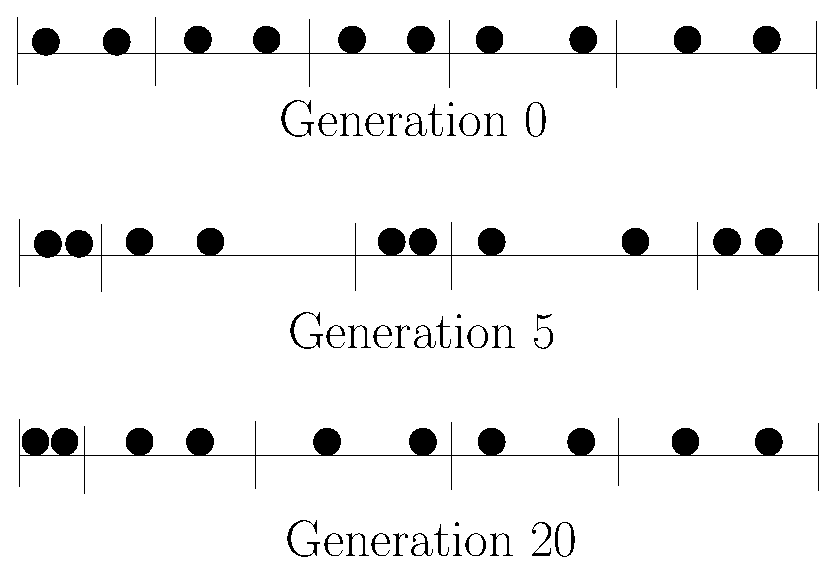
\includegraphics[bb = 144 82 686 502, clip, scale = 0.5]{FHH.eps}
    \caption{Population distribution generations by generations in FHH}
    \label{fig:FHH} 
  \end{center} 
\end{figure}

Giving a fixed bin number, $k$, two traditional methods of
discretization are fixed height histogram (FHH) and fixed width
histogram (FWH)~\cite{tsutsui2001evolutionary}.
The first splits the domain according to the solution number within a
bin.
In other words, each region should be with the same number of solutions.
The solutions in the same region are encoded as the code assigned to the
bin.
The word \textit{height} here refers to the fixed number of the
candidates inside each bin.
We give an example in Figure~\ref{fig:FHH}.
The picture illustrates the change of the distribution of bins and
solutions starting from the initial.
Assume the population size = $10$ and $k = 5$, as the optimizer
correctly executes, the promising regions are recognized and become
narrower generations by generations.
We can tell from the sample that at the beginning, individuals and bins
are uniformly distributed.
As time goes by, some of the bins are considered better and thus reduced
the width to reach a high resolution.
Nevertheless, FHH still maintains the same number of solutions in each
bin in order to avoid losing diversity. \\
\begin{figure}[h] \begin{center}
    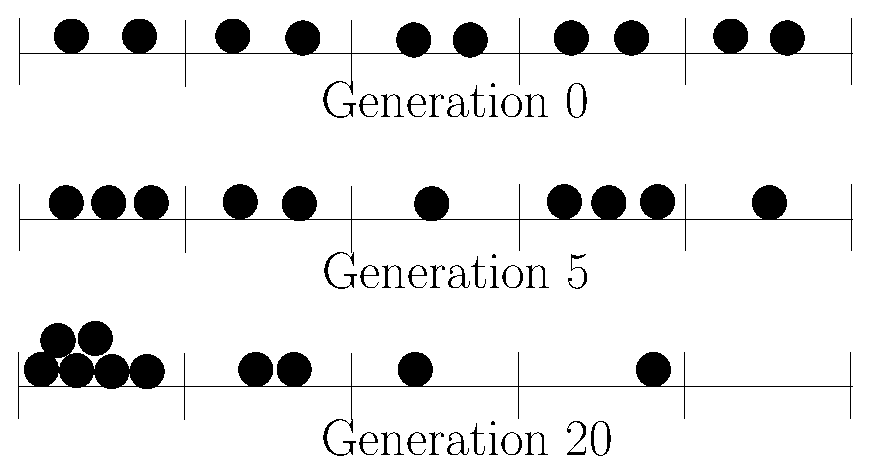
\includegraphics[bb = 144 82 686 502, clip, scale = 0.5]{FWH.eps}
    \caption{Population distribution generations by generations in FWH}
    \label{fig:FWH} 
  \end{center} 
\end{figure}
FWH, however, splits the domain according to a fixed length for which
the term \textit{width} stands.
Suppose there is a region in $\left(a,b\right]$ with $k$ bins, the
length of each bin is $\ell = \frac{b-a}{k}$.
Then the $i$-th bin is in the range $\left(a + (i-1)\ell ,
a+i\ell\right]$, where $i \in \left\{ 1,2,\ldots, k\right\}$.
Again, a simple example for FWH is given in Figure~\ref{fig:FWH}.
With identical settings to FHH, FWH starts with uniformly sampled
population.
Unlike FHH, the boundaries of each bin never changes.
After some generations, as the better regions are recognized, the newly
sampled solutions are concentrated in the promising regions. 
This may lead to a premature convergence due to the lost of solutions in
the region of less probability to find out global optimum.
Furthermore, a region never condenses is hard to reach high resolution
results.

\subsection{SoD} \label{sec:SoD} To make it compatible with real-valued
function optimization problems, in 2006, Chao-Hong Chen \textit{et al}.\ proposed
the real-coded extended compact genetic algorithm
(rECGA)~\cite{chen2006adaptive}, which supplies a solution to continuous
problems.  The basic idea of the
proposed rECGA is the adaptive segmentation and integer coded on the
domain of each decision variable.  By segmenting the continuous domain
with integer codes, the problem is changed from searching a solution to
searching a promising region.

The discretization method applied by the proposed rECGA, Split-on-Demand
(SoD), is different from traditional methods described above.  SoD and
FHH are similar in the concept that an area is decided to split based on
the information of density.  However, unlike FHH, SoD does not define a
fixed density of a region; instead, SoD sets a criteria that the density
of each region should not exceed a percentage $\gamma$.  Once a region
is found to have too many solutions inside, it is cut into two, with a
random selected bound between the upper bound and lower bound of the
region, and the discretion process is executed recursively on each newly
split region until there is no invalid region which exceeds the density
threshold.  In SoD, the threshold $\gamma$ decays with a factor
$\epsilon$.  The reason why $\gamma$ should decay is that higher
$\gamma$ is needed in the beginning to implement a more roughly global
search, but at late stages, SoD requires a smaller $\gamma$ to implement
a more fine model for local search. 

The detail algorithm of SoD is given in Algorithm~\ref{algo:SoD}, and
the algorithm of rECGA with SoD is given in Algorithm~\ref{alg:rECGA}.
\begin{algorithm}  {
    \KwIn{$upper\_bound$,$lower\_bound$}\ \Begin {
    Split($upper\_bound$,$lower\_bound$)\; $\gamma = \gamma
  \times\epsilon$\;} \Begin(Split) { mid = $random(high,low)$\; rateHigh
    =	$individualsNum(high,mid) / N$\; rateLow =
    $individualsNum(mid,low) /N$\; \If{rateHigh \textgreater $\gamma$} {
    Split(high,mid)\;   } \Else { AddCode(high,mid)\;    } \If{rateLow
    \textgreater $\gamma$} { Split(mid,low)\;     } \Else {
    AddCode(mid,low)\; } } } \caption{SoD} \label{algo:SoD}\end{algorithm}

\begin{algorithm}  \caption{rECGA with SoD} \label{alg:rECGA}Initial
  population\; \While{model is not converged} { perform tournament
    selection\; encode each dimension by executing SoD\; model the
    population by greedy MPM search illustrated above\; generate
  offspring\; perform local search on top 10\% individuals every L
generation } \end{algorithm} 

According to the proposed algorithm, rECGA first applies SoD to encode
legal regions of each dimension, and then applies ECGA to locate where
global optimum might be precisely; in the end, it applies Simplex, a
local search method, to observe higher resolution candidates.  In the
algorithm, ECGA is important for its ability of model building, which
significantly reduces the cost of exploring regions for rECGA by
eliminating regions where the global optimum is impossible to exist.

\section{Covariance Matrix Adaptation Evolution Strategy}
\label{sec:CMA-ES}


\subsection{Evolution Strategy} \label{ES}

Evolution Strategy (ES) is an instance of Evolutionary Algorithm from
the field of Evolutionary Computation and is most commonly applied to
black-box optimization problems in real search space.  They belong to
the family of Evolution Algorithm which solves problem by repeating a
process of stochastic variations followed by selection.  Despite being
inspired by biological evolution, ES lays emphasis on the mutation
operator.

Briefly speaking, the main idea of ES is to generate new solutions
iteratively by mutation on current solutions and replace old solutions
under selection.  Here the repeated process of each iteration in ES is
formulated and the notations will be described below

  \[\vec{x_i} \leftarrow m + \sigma N_i(0,\mathcal{C}),\]
where $i = 1,2,\ldots, \lambda$.


\begin{center}
  \begin{tabular}{|>{\centering} m{0.7in} | m{4.2in}|} \hline
    $\vec{x_i}$    & $\vec{x_i}$ is the \textit{i}-th generated
    offspring and denoted as vector.\\\hline $m$      & The mean vector
    m is mean of current solutions.\\\hline $\sigma$ &  $\sigma \in
    \mathbb{R}_+$ is the so called \emph{step size}.\\\hline $N_i$    &
    $N_i$ is the \textit{i}-th multivariate Gaussian perturbation
    according to C.\\\hline $C$      & A positive definite $\ell \times
    \ell$ matrix $C$ represents the shape of possibly region in which
    offspring of next generation should be.$\ell$ here indicates the
    number of decision variables\\\hline $\mu,\lambda$ & $\mu$ is the
    \emph{parent size} while $\lambda$ is the \emph{offspring
    size}\\\hline \end{tabular} \end{center}

We can now tell from the formulation that the mechanism of mutation is
to add random noise drawn from normal distribution to each vector
component.  To generate solutions, ES first takes the central of the
current population, usually weighted arithmetic mean of vectors, as the
point to sample from.  Normal distribution is taken as noise generator
because of the property that (1) normal distribution is widely observed
in nature, (2) normal distribution takes almost no assumption on the
object function and (3) normal distribution is the easiest way to
generate isotropic points.  That is to say, applying normal distribution
as noise generator favors no direction.  After mutation, selection takes
place at the end of each iteration; $\mu$ outstanding individuals are
selected out of the candidate pool as the parent of next generation.
The routine keeps executing until termination criteria, a limit number
of function evaluation for example is met.

Two well-known types of ESs are ($\mu, \lambda$)-ES and ($\mu+\lambda$)-ES\@.  The difference between them is that ($\mu,
\lambda$)-ES selects new $\mu$ candidate solutions from $\lambda$
generated solutions, while ($\mu+\lambda$)-ES selects new
$\mu$ candidate solutions from the union of original population and
$\lambda$ generated solutions.  Under the mechanism, there are different
properties for each: ($\mu+ \lambda$) selection is an elitist strategy,
where good solutions are always kept in the population; on the other
hand, ($\mu,\lambda$) selection always abandons good solutions have been
found so far.  The latter is preferred because that in elitist
strategies, a bad step size is difficult to update to a fine one if
there is a very fit solution.  In other words, ($\mu, \lambda$)
selection strategies make it easy to leave local optima.

\subsection{Methodology}

According to the template of ES, however, there are various modification
on step size $\sigma$ and covariance matrix $C$.  Among the branches of
ES, covariance matrix adaptation evolution strategy (CMA-ES) is the
famous one for its ability of evolutionary $\sigma$ and $C$.  In the
following the importance along with the modification will be introduced.

\subsubsection{Step size}

The step size $\sigma$ is adaptively adjusted according to the quality
of generated solutions.  This idea comes from the concept that a search
method is suggested to maintain its ability of exploitation and
exploration simultaneously.  With smaller step size, the search usually
digs out high resolution solutions nearby better, which is so called the
ability of exploitation.  In contrast to exploitation, the ability of
exploration stands for the ability to find out undeveloped region in the
search space, and higher step size helps the search with it.

It is not applicable to choose a fixed step size for the whole
optimization cycle for real-valued function optimization problems.  In
early stages of the search, we should avoid searching in a limited small
area and probe into the region that has not been reached yet, and this
implies the ability of exploration is far more vital at the early stage
of search.  On the other hand, the ability of exploitation is more
essential in the late stage.  With convincing overview, the optimization
converges to an appropriate region and would like to drop more efforts
here to generate more suitable solutions.  Under this situation,
exploration is no longer needed and the search now focuses on finding
better solutions nearby, which requires better ability of exploitation.
To sum up, there is a trade-off between exploration and exploitation and
the situation differs in each generation, and the step size is the
factor which controls the proportion and thus adaptively changes value
according to the environment.

Here we provide a simple instance for adaptively changing $\sigma$.  It
is named `One-Fifth success rule' and can be formulated as below.

\begin{center} {$\sigma \leftarrow \sigma \times \exp^{\left(
    \frac{1}{3} \times \frac{P_s-P_t}{1-P_t} \right)},$}\\ \end{center}
  where $\sigma$ is initial to $1$, $P_s$ stands for the proportion of
  offspring that better than parent and $P_t$ is the target probability
  $\frac{1}{5}$.  We can observe from the formula that once $\sigma$
  decreases or increases depends on if $P_s < P_t$ or not.

  CMA-ES applies a more complicated method by considering the cumulative
  path of the movement of the central $m$.  The basic concept behind is
  as described above.  There is an estimation of the cumulative
  evolution path so that we can observe the length of the vector, which
  indicates the path central really moved.  If the central moves
  slightly, it means the step size is too large to improve the
  population well, and $\sigma$ decreases accordingly.  On the other
  hand, if the central moves in vast, CMA-ES would suggest a larger step
  size to increase the exploration.

  To sum up, we can formulate the update of the $\sigma$ as following:\\
  \begin{center} {$p_{\sigma} =
    (1-c_{\sigma})p_{\sigma}+\sqrt{1-{\left(
      1-c_{\sigma}\right)}^2}\sqrt{\mathbf{\mu_w}}\mathbf{y_w}$\\
      $\sigma = \sigma \times \exp^{ \frac{c_{\sigma}}{d_{\sigma}}
      \left(\frac{\left|| p_{\sigma} \right||}{
        E\||{\mathcal{N}(0,I)}\||} -1 \right)  },$\\ } \end{center} where
      $p_{\sigma}$ is the cumulative evolutionary path initial to
      $\vec{\textbf{0}}$, $c_{\sigma}$ and $d_{\sigma}$ are pre-defined
      constants, $\mathbf{\mu_w}$ is the sum of the inverse squared
      weight of generated solution, and $\mathbf{y_w}$ is the weighted
      sum of noise generated .  \subsubsection{Covariance matrix} Recall
      the term `linkage' we discussed in the previous section, there are
      dependency between $n$ decision variables.  As we mentioned, ES
      takes covariance matrix to represent this dependency.  Since the
      linkage may not be simple, the covariance matrix is not supposed
      to be a diagonal matrix, and this makes it difficult to sample
      variables separately.  On the viewpoint of linear algebra, we are
      able to perform eigen decomposition on the matrix so that we just
      have to sample$n$ 1-D numbers by variance of each.  That is to
      say, by rotating the coordinates, $C$ is able to transfer into a
      diagonal matrix and thus it is now easy to sample according to the
      rotated variance of each variable.

  Recall the formula of ES that \[ x_i \leftarrow m + \sigma
  N_i\left(0,\mathcal(C)\right),\] where $i = 1,\ldots,\lambda.$\\ if we
  sort the generated solution according to fitness and re-encode each
  solution so that \begin{center} $f(x_{1:\lambda}) \leq
    f(x_{2:\lambda}) \leq \ldots \leq f(x_{\lambda:\lambda})$
  \end{center} and each is with weight $w_i$. Then the new average
  \begin{center} $m' \leftarrow \sum\limits_{i=1}^{\mu} \left(w_i
    x_{i:\lambda}\right) = m + \sum\limits_{i=1}^{\mu}w_i
    N_{i:\lambda}(0,C) = m + \sum\limits_{i=1}^{\mu}w_i y_{i:\lambda} =
    m + \mathbf{y_w}$ \end{center} CMA-ES is famous for the ability of
  adaptation for covariance matrix.  There are two options for updating
  the matrix: using historic information or using the selected
  individuals.  The former collects the cumulative information and the
  main target is to increase the likelihood of successful steps,
  $\mathbf{y_w}$, to appear again.  The latter focuses on the current
  selected individuals.  With a number of candidate solutions and the
  rank between them, there should be convincing dependency information
  inside, and the adaptation tries to dig out.  According to the
  property illustrated, the first one can learn from evolutionary path,
  thus a small population is enough and the number of function
  evaluations decreases.  The second, however, needs a proper size of
  population to extract current information  thus less generation needed
  than the first.

      CMA-ES combines the feature of both and can be formulated
      accordingly 
      \begin{center} 
        $\mathbf{{P_c}} = (1-c_c)\mathbf{{P_c}}+\left\{
          \begin{array}{ll}
          \sqrt{1-{\left(1-c_c\right)}^2}\sqrt{\mu_w}{\mathbf{y_w}} &
          \quad \text{if $\|\mathbf{p_{\sigma}}\| < 1.5\sqrt{n}$}\\ 0 &
          \quad \text{otherwise }
        \end{array}
        \right.$\\ $\mathcal{C}' = (1-c_1-c_{\mu})\mathcal{C} +
        c_1{\mathbf{P_c}}{\mathbf{P_c}}^T +
        c_{\mu}\sum\limits_{i=1}^{\mu}
        w_i\mathbf{y_{i:\lambda}}\mathbf{y_{i:\lambda}}^T, $ 
      \end{center}
      where $c_1$ , $c_c$and $c_{\mu}$ are constants, $\mathbf{P_c}$,
      initial to $\mathbf{0}$ is the cumulative information of
      evolutionary path, $n$ is the number of decision variables, and
      $\mathbf{y_i}$ is the generated noise of rank \textit{i} offspring

          We could tell from the equation that the first addend is the
          decadence of the originally covariance matrix while the second
          and the third addends perform the effect of history based
          information and population based information respectively. By
          combining the three factors along with proper weights, the
          proposed method makes the covariance matrix self-adaptive. 

          To sum up, we are going to give a detail procedure for the
          CMA-ES in Algorithm~\ref{algo:cmaes}:

\begin{algorithm} 
  \KwIn{$\mathbf{m}\in\mathbb{R}^n$,$\sigma\in\mathbb{R}$, $\lambda$}
  Initialize: $\mathcal{C} = \mathbf{I}$, $\mathbf{P_c} = \mathbf{0}$,
  $\mathbf{P_\sigma} = \mathbf{0}$\; Set: $c_c = \frac{4}{n}$, $c_\sigma
  = \frac{4}{n}$, $c_1 = \frac{2}{n}$, $c_\mu = \frac{\mu_w}{n}$,
  $d_\sigma = 1+\sqrt{\frac{\mu_w}{n}}$,\\sorted weight
  $w_1,w_2,\ldots,w_\lambda$ such that $\mu_w =
  \frac{1}{\sum\limits_{i=1}^\lambda w_i^2}\approx 0.3\lambda$ \;

  \While{not terminate} { \underline{\textbf{Sampling}} : $\mathbf{x_i}
  = \mathbf{m} + \sigma \mathbf{y_i}$, $\mathbf{y_i}
  \sim\mathcal{N}_i(0,\mathcal{C}),$ $i = 1,\ldots,\lambda$\;
  \underline{\textbf{Updating}} : $\mathbf{m} \leftarrow
  \sum\limits_{i=1}^\mu w_i \mathbf{x_{i:\lambda}} = \mathbf{m}+\sigma
  \mathbf{y_w}$, where $\mathbf{y_w} = \sum\limits_{i=1}^\mu w_i
  \mathbf{y_{i:\lambda}}$\; \underline{\textbf{Cumulation for matrix}}
  : $\mathbf{P_c} = (1-c_c)\mathbf{P_c}+\left\{ \begin{array}{ll}
    \sqrt{1-{\left(1-c_c\right)}^2}\sqrt{\mu_w}{\mathbf{y_w}} &
    \quad \text{if $\|\mathbf{p_{\sigma}}\| < 1.5\sqrt{n}$}\\ 0 & \quad
    \text{otherwise} \end{array}
  \right.$\; \underline{\textbf{Cumulation for step size}} :
  $\mathbf{p_{\sigma}} =
  (1-c_{\sigma})\mathbf{p_{\sigma}}+\sqrt{1-{\left(
    1-c_{\sigma}\right)}^2}\sqrt{\mathbf{\mu_w}}\mathcal{C}^{-\frac{1}{2}}\mathbf{y_w}$\;
    \underline{\textbf{Adaptation for matrix}} : $\mathcal{C} \leftarrow
    (1-c_1-c_{\mu})\mathcal{C} + c_1{\mathbf{P_c}}{\mathbf{P_c}}^T +
    c_{\mu}\sum\limits_{i=1}^{\mu}
    w_i\mathbf{y_{i:\lambda}}\mathbf{y_{i:\lambda}}^T$\;
    \underline{\textbf{Adaptation for step size}} : $\sigma = \sigma
    \times \exp^{ \frac{c_{\sigma}}{d_{\sigma}} \left(\frac{\left||
      p_{\sigma} \right||}{ E\||{\mathcal{N}(0,I)}\||} -1 \right)  }$\;
    } \caption{CMA-ES} \label{algo:cmaes}\end{algorithm}

\section{Thesis objective} \label{sec:motivation}

In this section, we are first going to illustrate the
hazard which may occur when processing CMA-ES for
optimization.
After understanding the difficulty to apply CMA-ES to real-valued
function optimization, we are going to describe the inspiration of the
thesis and construct a hypothesis to obtain a more fine evolutionary
algorithm.
\subsection{Difficulty of CMA-ES} Being an outstanding local optimizer,
CMA-ES performs well on figuring out solutions in a restrict region.
This property, however, leads CMA-ES to a premature convergence when the
search space grows largely. 

We can first take a look at the Figure~\ref{fig:localExample} to
illustrate the described hazard.
\begin{figure}[h] \begin{center}
    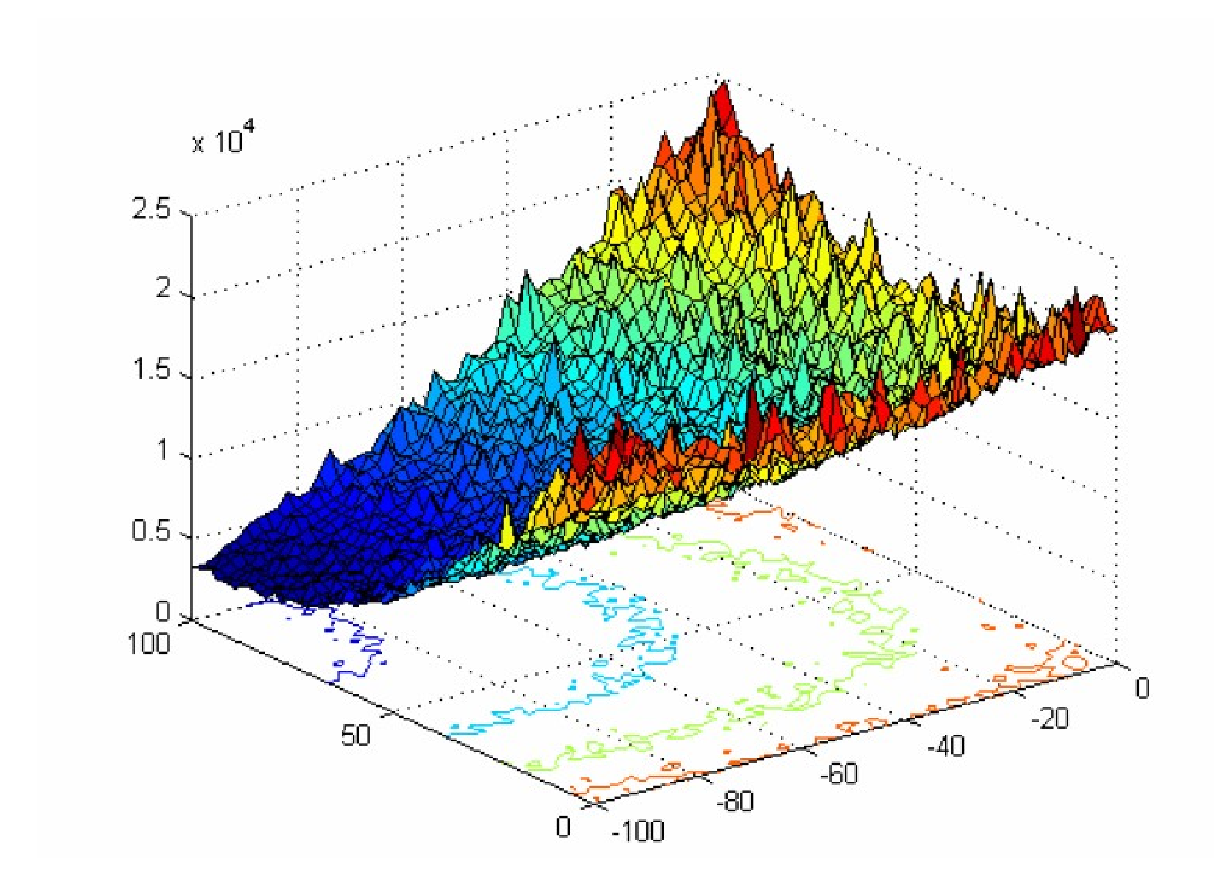
\includegraphics[scale = 0.5]{2Dproblem3DMap.eps}
    \caption{Example for local optima}
    \label{fig:localExample} 
  \end{center} 
\end{figure}
This is an example for fitness landscape of 2-D
function, and the goal is to minimize the function
value.  From the shown distribution of fitness we can
imagine that there should be a number of valley, which
we refer to as local optimum, in real-valued
optimization problems.  With a small population, it is
impossible to reach global optimum unless the initial
population are just sampled right around the best
valley.  Due to the rugged property of real-valued
optimization problems, CMA-ES being a good local
optimizer is just easily trapped in one of the local
optima.

  Generally in evolution algorithm, the most popular
  solution to the hazard is increasing the population
  in order to observe a high diversity.  CMA-ES,
  however, obtains no benefits from the method.  The
  reason can be distinguished by the mechanism of
sampling.  If a huge population is applied and
sampled uniformly, it can only be said that the mean
vector comes closer to the central of the search
space.  However, the population size affects only
the initial position of the mean vector $m$.  As the
routine starting to execute, the population size
turns to be useless because it is $\mu$ and
$\lambda$ that controls the size of evolution.  At
the second generation, $m$ is updated by the
weighted mean of selected solutions, which was
affected not only initialed $m$ but initialed step
size, initialed covariance matrix, etc.  That is to
say, with a huge amount of initial population, the
only affected condition is that the expected
distance of $m$ and the center of search space
becomes shorter.  The evolution path are then driven
towards the region where the fit solutions are in
the early stage, and this means the property of
diversity we wish to obtained according to a huge
population size is not useful under the mechanism.

\subsection{The hypothesis to conquer the
                    difficulty}

The original form of CMA-ES faces the problem
described above.  To conquer the difficulty of
\emph{non-convex}, the first idea comes from that if
we are able to roughly estimate the region where the
global optimum locates.  Once there is just a small
region, CMA-ES is believed to be capable of finding
out the optimum inside.  The technique of estimation
can be built in many ways.  For example, in
Section~\ref{sec:rECGA} rECGA applies discretization
to reduce the search space from an infinite,
continuous space to a finite, discrete space.
Followed with model building to distinguish the
region where the global optimum may locate.

Inspired from the concept of discretization, we
consider it possible to increase the performance of
CMA-ES when dealing with \emph{non-convex} problems.
Since CMA-ES majors in finding local optimum while
rECGA is famous for the ability to extract linkage
information, we don't think it appropriate to
integrate SoD directly into CMA-ES.  To be detail,
the reason can be described that local optimizer is
only taken every $L$ generations in rECGA, which
means the power of local optimizer is not the
definitive factor which affects the performance of
rECGA.

Since CMA-ES is with the ability to converge fast,
observing a valley is kind of easy job.  That is to
say, CMA-ES makes it fast to converge in one region.
Based on the property of good performance in
exploitation, the template of our hypothesis is
illustrated in the following.  To conquer the
\emph{non-convex} problem, a large population is
again sampled uniformly in the search space.  As
described, the native CMA-ES is not able to take
advantages from the diversity.  Therefore, we divide
these huge population into several groups.  Being an
outstanding optimizer, CMA-ES can easily evaluate
local optimum of each group.  The main assumption is
that the information of global optimum can be
extracted from these groups.  To be precise, by
evolving each group under some specific order and
choosing a representative solution for the
distribution, we wish to evolve the set consists of
representative solutions according to some method
and then reach the cliff as close to the global
optimum as possible.

To sum up, the hypothesis wishes to benefit from the
diversity brought by a large population.  Inspired
by discretization, we divide the population into
groups in order to keep diversity.  An approach
should be supplied to communicate among the groups,
thus we are able to take advantages from the
discretization. Instances of the hypothesis will be
proposed in the next chapter.  
